%%%%%%%%%%%%%%%%%%%%%%%%%%%%%%%%%%%%%%%%%%%%%%%%%%%%%%%%%%%%%%%%%%%%%%%%%%%%%%%%
% simulation.tex: Chapter on ECAL Timing
%%%%%%%%%%%%%%%%%%%%%%%%%%%%%%%%%%%%%%%%%%%%%%%%%%%%%%%%%%%%%%%%%%%%%%%%%%%%%%%%
\chapter{Timing Reconstruction and Calibration}
%%%%%%%%%%%%%%%%%%%%%%%%%%%%%%%%%%%%%%%%%%%%%%%%%%%%%%%%%%%%%%%%%%%%%%%%%%%%%%%%
The time of an electromagnetic object such as a photon is extracted at the level of individual crystals called reconstructed hits~(rechits). The recorded time of the photon is the crystal calibrated time where the Time-Of-Flight~(TOF) as well as the time to transmit the recorded signal from the front-end detectors to the back-end readout electronics is removed such that on average the time is zero for a photon produced at the nominal proton-proton collision point and travelling at speed of light and then impinges at the surface of the crystal.  There are separate algorithms for extracting and calibrating the crystals using the rechit time. This calibrated time is considered the reconstructed time~($T_{RECO}$). 
Measuring the difference in timing between any two reconstructed objects ( individual crystals or electromagnetic objects) originating from the same nominal point and thus assumed in principle to have the same time give the timing resolution of the detector as well as the crystal-to-crystal synchronization factor.  $T_{RECO}$ of a photon can be defined in either of the following ways:
\begin{enumerate}
\item Seed Time: The time of the highest energy crystal or rechit in the highest energy basic cluster of the photon supercluster denoted as $T_{SEED}$
\item The Mean Time: This is the error weighted mean time of all the crystals in the photon supercluster denoted as $T_{CLUSTER}$ or $T_{MEAN}$ and is defined as follows:
\begin{equation}
T_{CLUSTER} = T_{MEAN} = \frac{\sum_{i=1}^N\frac{T_{i}}{\sigma_{i}^{2}}}{\sum_{i=1}^{N}\frac{1}{\sigma_{i}^{2}}} 
\end{equation}
\newline
 where N is the number of crystals in seed basic cluster of photon supercluster. 

\end{enumerate}
\subsection{Electromagnetic Calorimeter Readout Chain}
%%%%%%%%%%%%%%%%%%%%%%%%%%%%%%%%%%%%%%%%%%%%%%%%%%%%%%%
The ECAL electronics readout system described in detailed in \cite{ECALREADOUT} is a light-to-light system. Energy from incoming electromagnetic objects is absorbed and converted into scintillating light by \pb crystals. This is received and converted into electrical signals by the avalanche photo-diodes. These electrical signals are digitized and finally converted back into light signals which is transported using optical fibres into the off detector electronics in the counting room at point 5. Thus one can easily classify the full readout chain of the ECAL electronics readout system as divided into an on-detector electronics and an off-detector electronics.
Both electronics system are connected by a 100~m optical fibre links. A simple picture of the readout chain is shown in fig{FIXME:Fig readout Chain}.

%%%%%%%%%%%%%%%%%%%%%%%%%%%%%%%%%%%%%%%%%%
The on-detector electronics reads a trigger tower consisting of $5\times5$ crystals in $\eta \times \phi$ in barrel~(EB) and \textit{supercrystals} in endcap~(EE). Five Very Front End~(VFE) boards ( reading out  data from 5 crystals each), one Front End boad~(FE) two~(EB) and six~(EE) Giga Optical Hybrids~(GOH), one Low Voltage Regulator~(LVR) board and a Mother Board~(MB) make up the complete on-detector electronics. Electrical Signals from the APDs~(EB) are accepted by the VFE which is equipped with a Multi Gain Pre-Amplifier~(MGPA), a 12-bit Analogue to Digital Converter~(ADC) and a buffer. The MGPA an Application Specific Intergrated Circuit~(ASIC) developed in 0.25~$\mu$m technology, pre-amplifiers, shapes and then amplifies the signals through three amplifiers with gains of 1, 6 and 12. For VPT~(EE), these signals first pass through a High Voltage~(HV)filter card which acts as a moderator separating very high voltages caused by the increase radiation in the EE. The full scale of the APDs and VPTs are 60~pC and 12.8~pC corresponding to $\approx$ 1.5~TeV and 1.6-3.1~ TeV respectively. The full shaping of the signal takes about 40~ns. The noise for gain 12 is about 8000$e^{-}$ for APD configuration and about 4000$e^{-}$ for VPT configuration. 
The 3 analog output signals of the MPGA are digitized in parallel by the multichannel 40~MHz, 12-bit ADC. This ADCs have an effective number of bits of 10.9. The highest non-saturated signal is selected as the output signal and reported as 12 bits of the corresponding ADC with 2 bits coding the ADC number. It is possible, that when the signal is saturated and wrong signal amplitude can be produced leading to am amplitude dependence of the readout time. This effect has been studied for Gain 1 and 6 transitions and the relevant corrections factors of timing produced and validated.
A schematics picture of the showing the readout chain of the FE with its MPGA and ADCs showing the shaping and digitization process can be seen in figure \eqref{readout}.

\begin{center}\label{readout}
\centering
\mbox{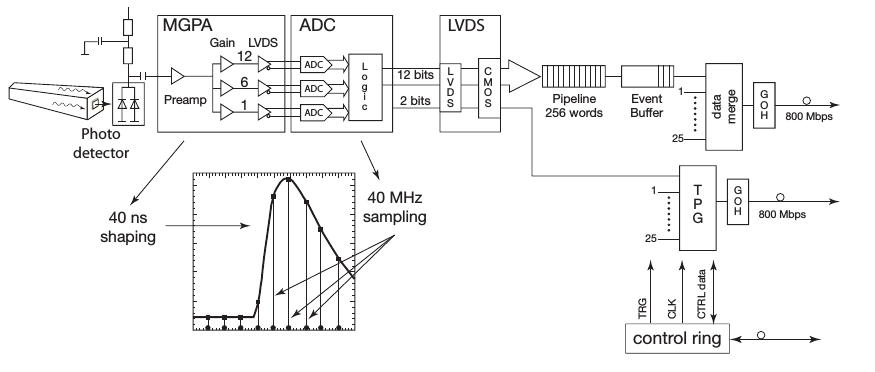
\includegraphics[scale=0.6]{/home/tensr/Documents/TEN-HEP-PHD-THESIS/PHD_THESIS/PHD/THESISPLOTS/ReadOut.png}} 
\captionof{figure}{Schematic showing ReadOut Chain.}
\label{fig:readout}
\end{center}

A radiation-hard buffer~(LVDS) adapts a low voltage differential out put signal of the ADC to input into the FE. Signals from  five  identical channels are integrated and read into VFE card with a Detector Control Unit for measuring  the APD leakage currents. The noise from each VFE is typically 1.1, 0.75, 0.6 ADC counts for gains 12, 6 and 1 respectively. This would be about 40~MeV for gain 12.

Digitized data from 5 VFE cards are fed into each FE through the LVDS and stored in 256-word-deep dual-ported memories called pipelines. Data pipelines can be stored for up to 128 bunch crossings. The FE is base on a ASIC called the FERNIX holding the logic to calculated the energy of 5 channels once every bunch crossing. This energy is summed in strips of 5 crystals  along $\phi$. Thus each VFE is serviced by a FERNIX chip. In the case of the EE, the five strip energy sum are transported by GOH to the off-detector electronics Trigger Concentration Card~(TCC) while for EB, there a sixth FERNIX which sums the five strips energy sums  and calculates an electromagnetic bit which is used to identify electromagnetic shower candidates on the basis of their shower profile in a trigger tower. The trigger tower energy sums and the electromagnetic bit is transmitted to the TCC through the GOH. This process is referred to as Trigger Primitive Genration~(TPG). Once a Level-1 trigger signal is received, the ten 40~MHz samples for each channel are transmitted to the off-detector electronics DCC using an identical GOH. This takes about 7.5~$\mu$s. The VFE and FE cards are controlled using a 40~MHz digital optical link system and controlled by the off-detector Clock and Control System~(CCS). 
The Off-detector electronics consist of different types of electronic boards~(the CCS, TCC and DCC modules) sitting in an 18 VME-9U crates and a 1 VME-6U crate holding the Selective Read-Out Processor~(SRP). This system is serving both the trigger and the  Data Acquisition Systems~(DAQ) paths. In the DAQ path, the DCC performs data read-out and data reduction based on flags of the SRP. While in the trigger path, at each bunch crossing, the trigger primitive generation which began in the FE is finalised and synchronised or time alignments in the TCC before transmitted to the regional calorimeter triggers. The trigger primitives each refer to a single trigger tower~(25 crystal data) and consists of  the summed transverse energy deposits and the electromagnetic bit charactering the lateral shower profile of the electromagnetic shower. The accept signal for accepted events is return from the global trigger after about 3~$\mu$sand the selected events area read into the data acquisition system to the filter farm where the even rate is further reduced using data from the full detector. Thus is the regional calorimeter, the ECAL trigger primitives  together with the HCAL trigger primitives are used to  compute the electron/photon and jet candidates as well as their transverse energy. The resulting physics objects after passing through the HLT trigger are transferred to the various tier systems for offline full event reconstruction. The ECAL also has a laser calibration systems where laser light is delivered directly to the \pb crystals using optical fibres. The laser data is used for energy and time calibration of crystals and hardware system. The crystals are energy calibrated because of the decrease in optical transmission due to the formation of color centres in the crystal. The formation of color centres is caused by irradiation. Time calibration using laser data is also required in case of hardware timing offset especially during long short down periods of the CMS detectors.
 %%%%%%%%%%%%%%%%%%%%%%%%%%%%%%%%%%%%%%%%%%%%%%%%%%%%%%%%%%%%%%%%%%%%%%%%%%%%%%%%
\subsection{Timing Extraction}
%%%%%%%%%%%%%%%%%%%%%%%%%%%%%%%%%%%%%%%%%%%%%%%%%%%%%%%%%%%%%%%%


The digital  filtering~(DF) technique is used to reconstruct the amplitude collected by the \pb crystals.
\begin{center}\label{CMSECAL}
\centering
\mbox{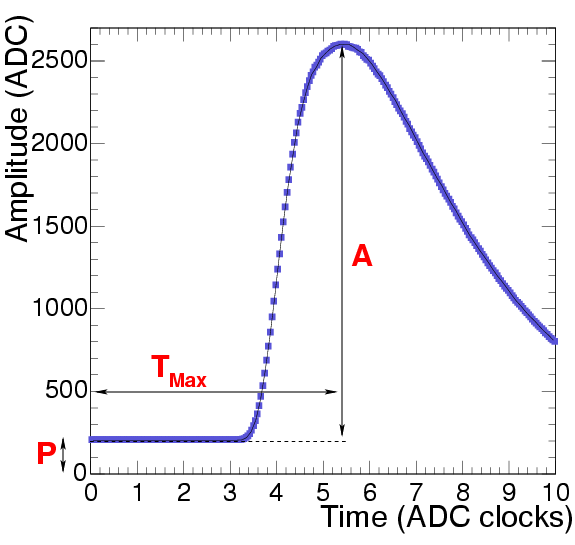
\includegraphics[scale=0.6]{THESISPLOTS/Time_Amplitude_Profile.png}}
%\mbox{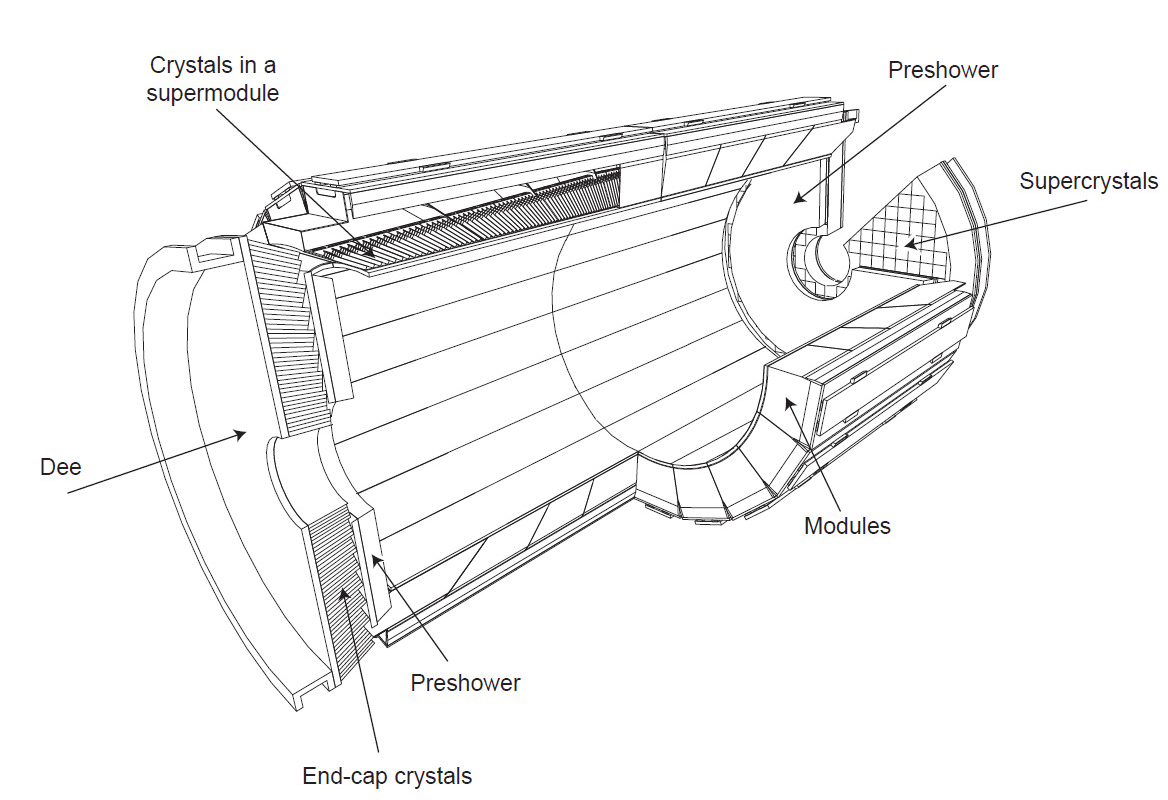
\includegraphics[scale=0.2]{THESISPLOTS/CMS-ECAL.png}}
%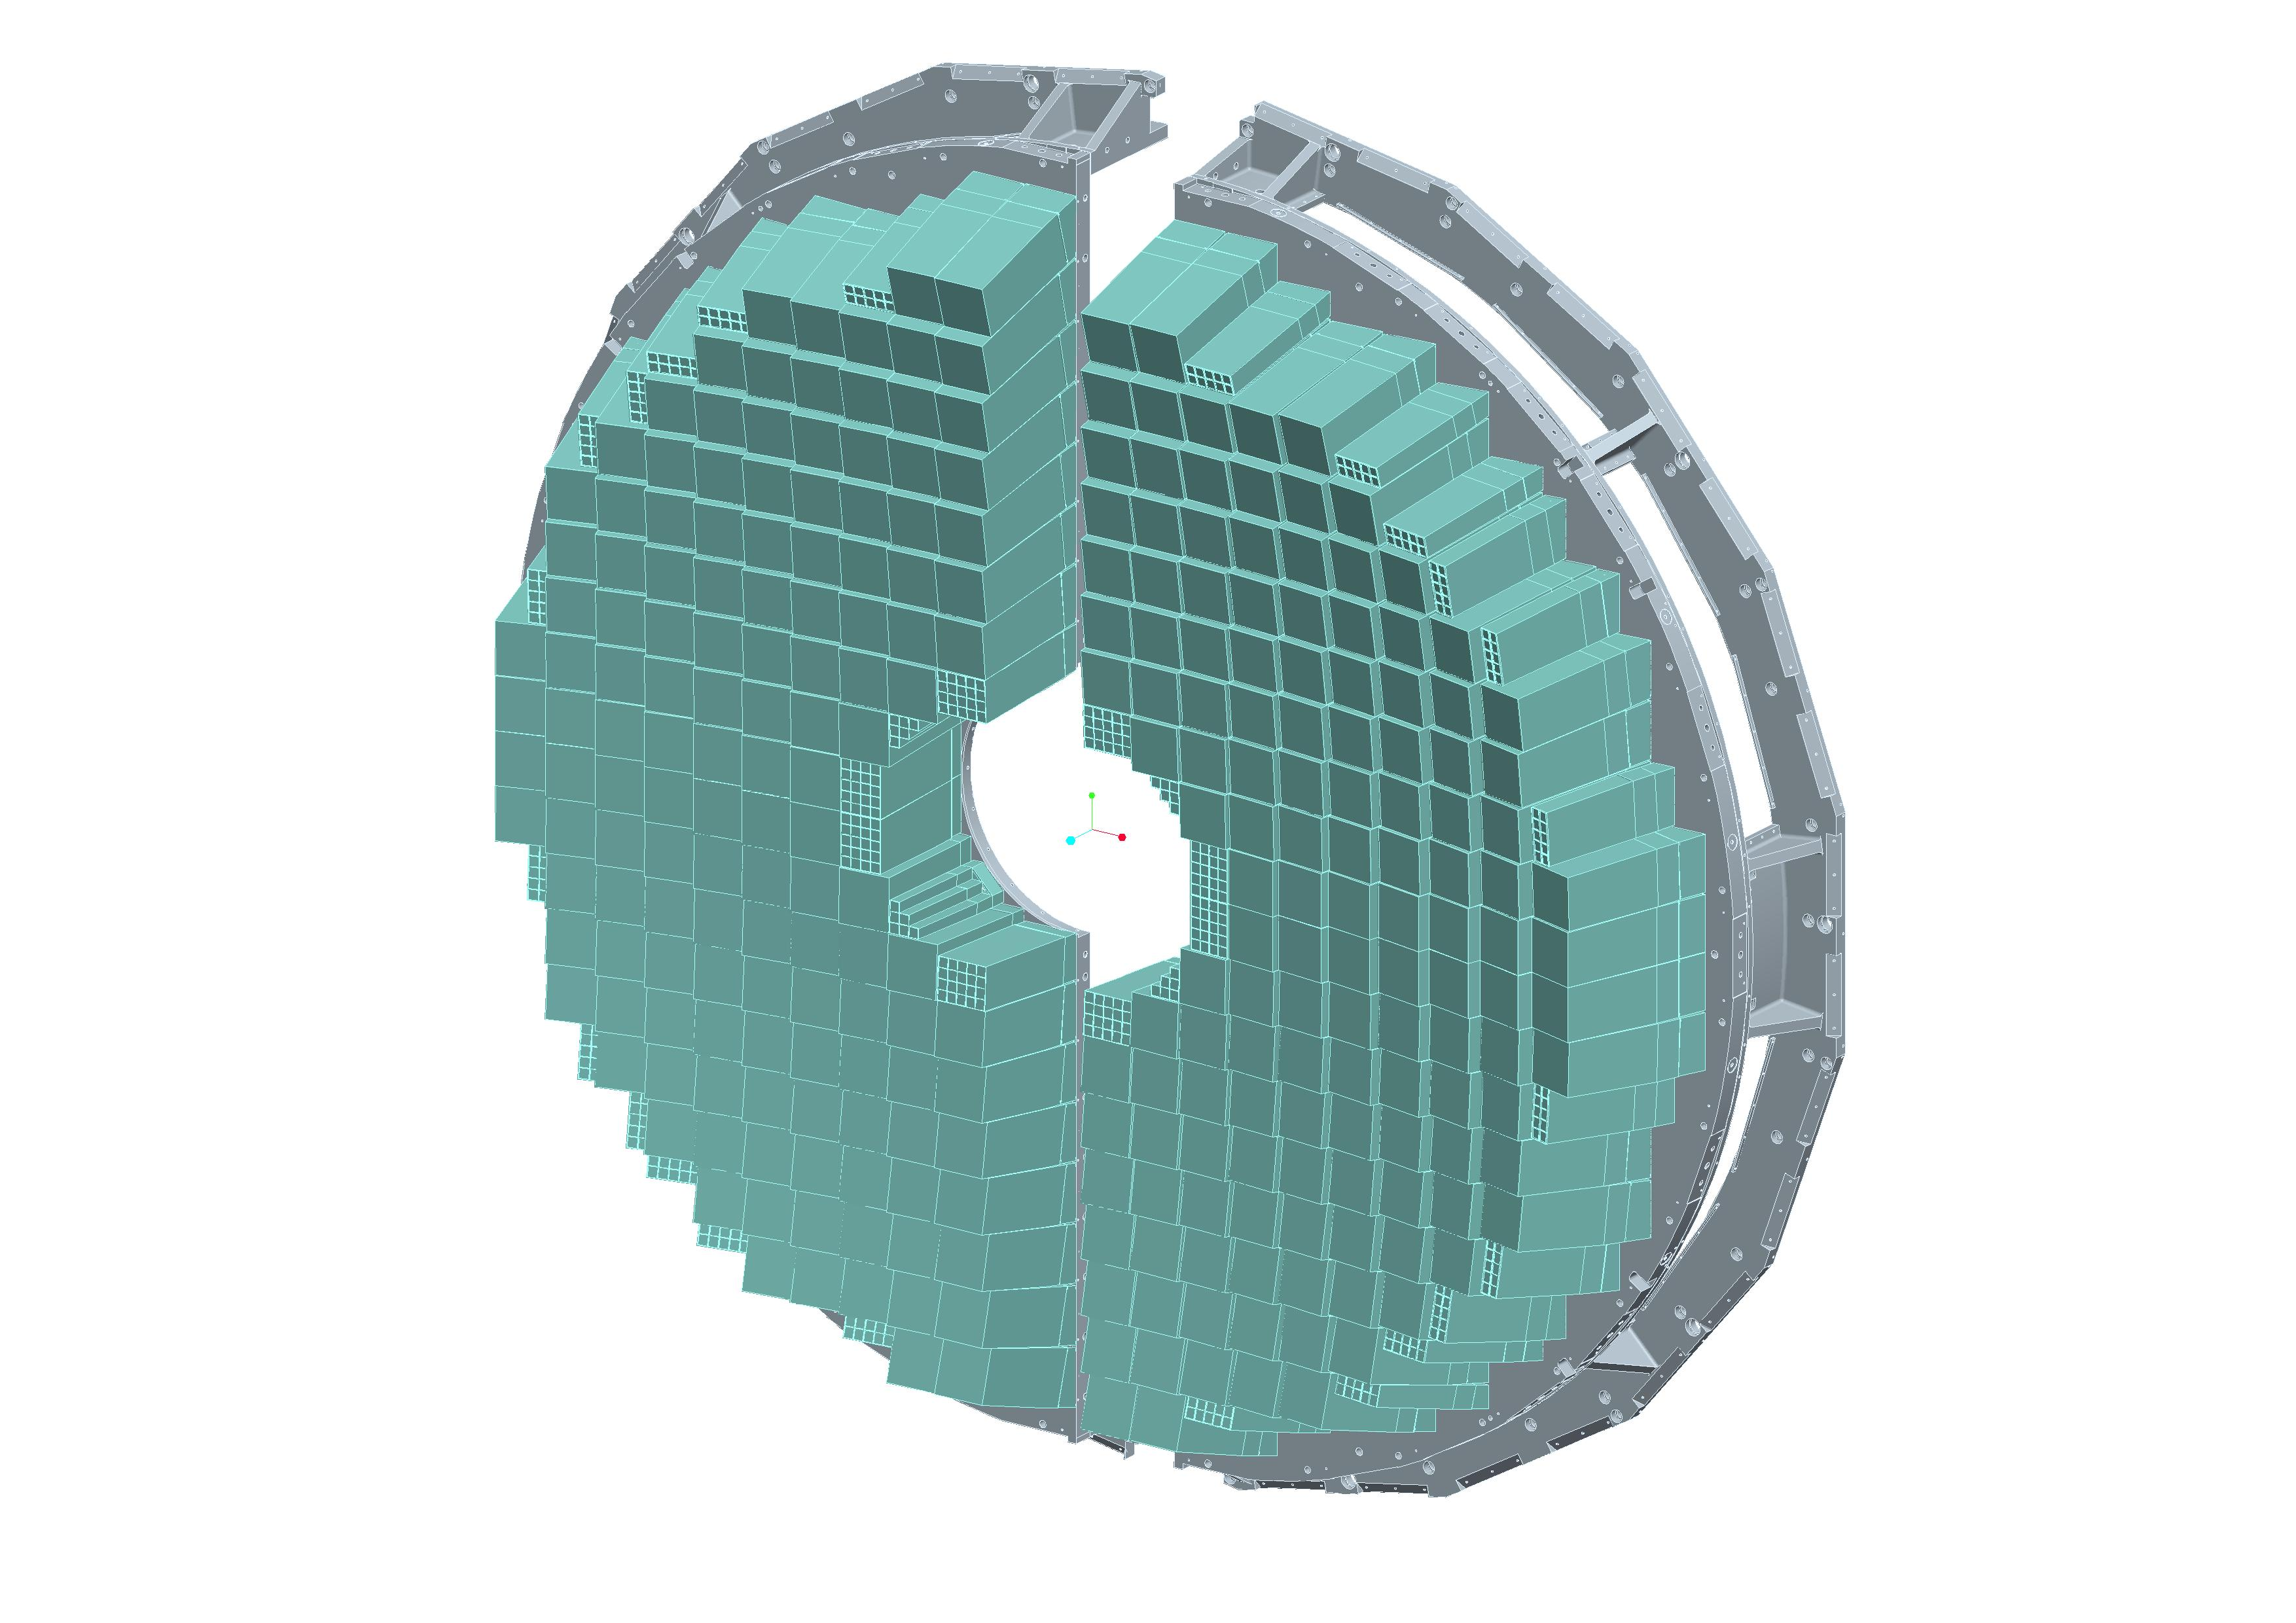
\includegraphics[scale=0.06]{THESISPLOTS/endcap_CMS.png}} 
\captionof{figure}{Typical pulse shape of a given signal showing signal amplitude and time.}
\label{fig:CMSECAL}
\end{center}
%%%%%%%%%%%%%%%%%%%%%%%%%%%%%%%%%%%%%%%%%%%%%%%%%
\subsection{Timing Calibration Procedure}
%%%%%%%%%%%%%%%%%%%%%%%%%%%%%%%%%%%%%%%%%%%%%%%%%%%%%
The Ecal time is calibrated such that the the time travel by a photon or any highly relativistic  particle  produce at the nominal region of CMS proton-proton collision is on average 0 ns. This ensures that if a particle in detected with a significantly large positive time, then it is either this particle is travelling with a very small velocity (slowly moving particles or small $\beta << 1$ particle or it was produced as the decay product of stopped particle in the detector or it is a particle which is not travelling in a straight line but rather on a curved path to reach the ECAL.


\subsubsection{HardWare Timing Calibration}
%%%%%%%%%%%%%%%%%%%%%%%%%%%%%%%%%%%%%%%%%%%%%%%%%%%%%%%%%%%%%%%%%%%


%%%%%%%%%%%%%%%%%%%%%%%%%%%%%%%%%%%%%%%%%%%%%%%%%%%%
\subsection{Electromagnetic Calorimeter Timing Performance}
%%%%%%%%%%%%%%%%%%%%%%%%%%%%%%%%%%%%%%%%%%%%%%%%%%%%%%%%%%%%%%%%%%
The time performance of the ECAL crystals is studied and validated using events with a Z decay  i.e $\PZ \rightarrow \Pelectron \Ppositron$. 
\newline
The main idea is to use two reconstructed "objects" which in principle should have the same time and then use their time difference as a measure of the timing performance. We:
\begin{enumerate}
\item use two crystals within the same electron super cluster.
\item use the two electrons from the $\PZ$ decay. 
\end{enumerate}
In using electron super clusters, we considered following additional contributions to the electron time:
\begin{enumerate}
\item The bending of the electron path due to the presence of the 3.8~T magnetic field of the CMS detector.
\item  Displaced collisions  because "partons"~(subparticles) in the protons of the proton-proton~(p-p) bunches did not collide at exactly the collision point or Nominal Interaction point~(IP).
\item The collision developed over the full duration of the overlap of the proton bunches.
\end{enumerate}

The Time-Of-Flight~(TOF) of the electron from the IP is considered in the time calibration algorithm of the ECAL crystals.
Indeed, one assumption of using photons to time calibrate the ECAL crystals in that, they travel with the speed of light and so on average the time taken for a photon to travel from the IP until it impinges on the crystal surface in on average 0. With this assumption true only for Nominal Collisions i.e collisions originating for the IP and travelling straight to the ECAL crystals.
\newline


\begin{center}
\centering
\mbox{
\includegraphics[width=3in]{/home/tensr/Documents/ECAL_NOTES/PLOTS/2013/ECALTDRPLOTS/EB-EB-Time-of-seed.png}\quad
\includegraphics[width=3in]{/home/tensr/Documents/ECAL_NOTES/PLOTS/2013/ECALTDRPLOTS/EE-EE-Time-of-Seed.png}}
\captionof{figure}{Ecal absolute time of a single reconstructed electron in $\PZ \rightarrow \Pelectron \Ppositron$ decay. The electron time is the seed~(crystal with highest energy deposit)time of the electron.(a) in in EB and (b) in EE} 
\label{fig:ZeeTimePerformance}
\end{center}

\begin{center}
\centering
\mbox{
\includegraphics[width=3in]{/home/tensr/Documents/ECAL_NOTES/PLOTS/2013/ECALTDRPLOTS/EB-EB-TOF-Corr-difference-of-seed.png}\quad
\includegraphics[width=3in]{/home/tensr/Documents/ECAL_NOTES/PLOTS/2013/ECALTDRPLOTS/EE-EE-TOF-Corr-difference-of-seed.png}}
\captionof{figure}{Ecal time difference between the two reconstructed electrons in $\PZ \rightarrow \Pelectron \Ppositron$ decay. The electron time is the seed~(crystal with highest energy deposit) time with additional correction due to the time of flight of the electron.(a) in in EB and (b) in EE} 
\label{fig:ZeeTimePerformance}
\end{center}
%\end{figure}

\begin{center}
  \begin{tabular}{|c|c|c|c|c|c|}
   \hline
   %table stuff \\
   \hline
  \end{tabular}
 \captionof{table}{Table Comparing Timing Resolution performance of 2011 Vs 2012}
   \label{table1} % for use in \ref{table1} if you want to refer to the table number
\end{center}

%%%%%%%%%%%%%%%%%%%%%%%%%%%%%%%%%%%%%%%%%%%%%%
\label{ECAL Timing Calibration_chapter}
